
%(BEGIN_QUESTION)
% Copyright 2008, Tony R. Kuphaldt, released under the Creative Commons Attribution License (v 1.0)
% This means you may do almost anything with this work of mine, so long as you give me proper credit

One of the most basic components of a pneumatic instrument is the so-called {\it flapper/nozzle}, or {\it baffle/nozzle} assembly.  It consists of two restrictions to air flow, one within a tube (the {\it orifice}) and the other at the end of a tube (the {\it nozzle}).  The {\it flapper}, or {\it baffle}, is nothing more than a flat piece of metal in close proximity to the nozzle tip.  These mechanisms serve as extremely sensitive position detectors, generating a pneumatic pressure output signal that varies with flapper (baffle) position:

$$\includegraphics[width=15.5cm]{i00191x01.eps}$$

Suppose that two pressure gauges were installed along the length of the tube, one upstream of the orifice and the other downstream of the orifice, like this:

$$\includegraphics[width=15.5cm]{i00191x02.eps}$$

Qualitatively speaking, what would these two pressure gauges indicate?  Assume that the air supply is regulated by a pressure regulator, and so remains at a constant pressure.  Would the two pressure gauges indicate the same amount of pressure?  Would one of them indicate a higher pressure than the other?  Explain your answer.

\vskip 10pt

If the flapper (baffle) is brought closer to the nozzle, the nozzle will become more restrictive to air flow through it.  What effect will this have on the two pressure gauge indications in this flapper/nozzle system?

$$\includegraphics[width=15.5cm]{i00191x03.eps}$$

\vskip 10pt

If the flapper travels further away from the nozzle, what effect will it have on the two pressure gauges' indications?

$$\includegraphics[width=15.5cm]{i00191x04.eps}$$

\underbar{file i00191}
%(END_QUESTION)





%(BEGIN_ANSWER)

The pressure gauge downstream of the orifice will indicate a lower pressure than the gauge upstream of the orifice.  Moving the flapper closer to the nozzle increases the downstream pressure, while moving the flapper away from the nozzle decreases the downstream pressure.

\vskip 10pt

Follow-up question: sketch a schematic diagram for an electrical circuit analogous to this pneumatic ``circuit'' formed by the pressure source, orifice, nozzle, and flapper.

%(END_ANSWER)





%(BEGIN_NOTES)

The upstream pressure will remain essentially constant, as regulated by the air pressure regulator installed upstream.

\vskip 10pt

Follow-up answer:

$$\includegraphics[width=15.5cm]{i00191x05.eps}$$

%INDEX% Basics, pneumatics: baffle/nozzle
%INDEX% Basics, pneumatics: flapper/nozzle

%(END_NOTES)


